\section{Register File Generation}\label{rf_generation}
RFs of state of the art hardware designs can easily contain several hundreds of CSRs. When an additional register is inserted during the design process, the entire address map of the RF has to be updated. Not only this has to be done in the hardware description, but also in all other parts involved in the design process like specification, documentation, and verification and simulation environment. This is both time-consuming and error prone. Therefore, it makes sense to have a single file containing the RF description with a high abstraction level. This file is then used to automatically generate all other required views.\\

Such RF descriptions can be drawn up using description languages like \emph{SystemRDL} or \emph{Spirit IP-XACT}, which are used in commercial RF generators. Where \emph{SystemRDL} is a language specific for RFs \cite{system_rdl} whereas \emph{Spirit IP-XACT} is not only able to describe RFs, but also the connections between hardware modules \cite{ip_xact}.\\

The main problem of these description languages is, that they do not support hierarchical RFs natively. When a single RF is placed centrally on a chip and the connected logic is spread across it, the routing delays between RF and logic become a huge concern. This can have a negative impact on the maximum frequency of the design. Hierarchical RFs can prevent this by placing the sub-RFs closer to the connected logic. Therefore the routing delays are reduced.\\
Additionally the syntax of both languages is not as clear as the one of the register file generator, which will be presented in the following section. Especially the one of \emph{Spirit IP-XACT} requires more characters to describe the same RF (fig.~\ref{fig::compare_syntax}).
\begin{figure}[h]
 \centering
 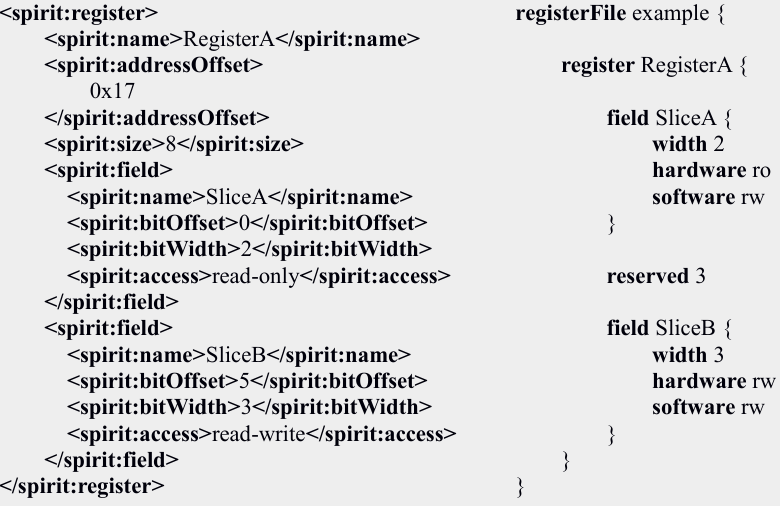
\includegraphics[width=252pt]{images/ip_vs_rfg.png}
 \caption{Spirit IP-XACT syntax compared to RFG \cite{markus_rfg}}
\label{fig::compare_syntax}
\end{figure}
